\documentclass[12pt, a4paper]{urjc}
\usepackage[left=3.5cm,top=2cm,right=3cm,includehead]{geometry}

\bibliography{bibliografia.bib} 

\newcommand{\grado}{}
\newcommand{\titulotrabajo}{Manual\\ DeduccionNatural.pl}
\newcommand{\asignatura}{Lógica}
\newcommand{\curso}{Curso 2022-2023}
\newcommand{\autorone}{Iván Ramírez}
\newcommand{\autortwo}{Joaquín Arias}
\newcommand{\autorthree}{}

\newcommand{\scasp}[1][]{\href{https://ciao-lang.org/playground/scasp.html}{\color{black}\faExternalLink*}}
\newcommand{\scaspaux}[3]{%
  \ifthenelse{\equal{#1}{#2}}{%
    \href{#3}{\color{saved}\faExternalLink*}%
  }%
  {}%
}
\renewcommand{\scasp}[1]{%
  \colorlet{saved}{.}
  \scaspaux{#1}{aristoteles}{https://bit.ly/3PXAsAM}%
  \scaspaux{#1}{concatenar}{https://bit.ly/3TjawT1}%
  \scaspaux{#1}{morse}{https://bit.ly/3Kk30mu}%
  \scaspaux{#1}{concatenar_b}{https://bit.ly/3cfvOAl}%
  \scaspaux{#1}{reach_a}{https://bit.ly/3QRy3IP}%
  \scaspaux{#1}{reach_b}{https://bit.ly/3KzWqc1}%
  \scaspaux{#1}{reach_acc}{https://bit.ly/3PRKFhS}%
  \scaspaux{#1}{reach_acc_scasp}{https://bit.ly/3KnBvbS}%
  \scaspaux{#1}{fibo}{https://bit.ly/3cqHeBc}%
  \scaspaux{#1}{hipoteca}{https://bit.ly/3cAhToi}%
  \scaspaux{#1}{deduccion}{https://tinyurl.com/deduccionnatural22}%
  % Default
  \scaspaux{#1}{}{https://ciao-lang.org/playground/index.html}%
}

\sloppy

%%%%%%%%%%%%%%%%%%%%%%%%%%%%%%% Inicio del documento
\begin{document}

\maketitle

\section{Introducción}

Este manual se enmarca en el contexto de la asignatura de Lógica en la
Escuela Técnica Superior de Ingeniería Informática de la Universidad
Rey Juan Carlos.

En concreto se centra en el aprendizaje de la Deducción Natural,
introducida por \citet{gentzen1935untersuchungen}.
%
La Deducción Natural busca capturar la manera en que las personas
razonan naturalmente al construir demostraciones matemáticas.
% 
En vez de contar con unos pocos axiomas a los que se aplican unas
pocas reglas de inferencia, la deducción natural propone vaciar la
lista de axiomas y ampliar la de reglas de inferencia, introduciendo
dos reglas para cada constante lógica ($\land$, $\lor$, $\lnot$,
$\rightarrow$, $\leftrightarrow$):
\begin{itemize}
\item Una para introducirla.
\item Otra para eliminarla.
\end{itemize}
Por lo tanto una demostración se construye partiendo de supuestos y
aplicando las reglas para llegar a la conclusión deseada.
%
Sirve para demostrar la validez de un argumento.

Para facilitar el aprendizaje hemos desarrollado una herramienta
usando programación lógica (disponible en
\url{https://github.com/Xuaco/DeduccionNatural}) que permite evaluar
si dada unas premisas y un consecuente, la demostración planteada por
el alumno es correcta. La fig.~\ref{fig:ded} muestra una captura de la
ejecución, en el Playground de Ciao\footnote{Ciao Prolog es un
  interprete de Prolog, disponible en \url{https://ciao-lang.org/},
  que cuenta con un Playground online en
  \url{https://ciao-lang.org/playground/index.html}}, del 
ejemplo~\ref{exa:eje}.

\begin{ejm}\label{exa:eje}
  Ejemplo extraído de los apuntes de \citet{arias22logica}.

  \medskip

\hspace*{-1.5em}\begin{minipage}[t]{.49\linewidth}
  Desarrollo con notación lógica:

  \bigskip

$T[s \land (p \lor q), p \rightarrow \lnot r, q \rightarrow \lnot
r] \vdash s \land \lnot r$

\[
  \begin{array}{lll}
    1. &  s \land (p \lor q)\hspace*{1cm} & premisa\\
    2. &  p \lor q & E_{\land} (1) \\
    3. &  p \rightarrow  \lnot r &   premisa\\
    4. &  q \rightarrow  \lnot r&  premisa \\
    5. &  \lnot r& E_{\lor} (2,3,4)  \\
    6. &  s& E_{\land} (1)\\
    7. &  s \land \lnot r & I_{\land} (5,6)\\
  \end{array}
\]

\end{minipage}
\vrule\hspace*{.25em}
\begin{minipage}[t]{.49\linewidth}
  Traducción en \code{DeduccionNatural.pl}:
  \hfill \scasp{deduccion}

  \medskip

\begin{lstlisting}[style=MyProlog]
ejemplo1 :-
    main([ s and p or q,
           p --> ! r,
           q --> ! r     ],
         s and ! r,
         [   'Premisa'(1),
             'E' and b(1),
             'Premisa'(2),
             'Premisa'(3),
             'E' or (2,3,4),
             'E' and a(1),
             'I' and (6,5)  ]).
\end{lstlisting}

\end{minipage}
\end{ejm}


A continuación, la Sección~\ref{sec:operadores} describe como se han
traducido los operadores y las reglas de inferencia. La
Sección~\ref{sec:deduccion} explica como ejecutar el programa para
comprobar si una demostración es correcta dado unas premisas y un
consecuente. Finalmente, la Sección~\ref{sec:derivadas} muestra como
definir reglas derivadas (o de usuario) para factorizar las
demostraciones.

\section{Constantes lógicas y reglas de inferencia}
\label{sec:operadores}


\section{Ejecución del programa}
\label{sec:deduccion}

\begin{figure}
  \centering
    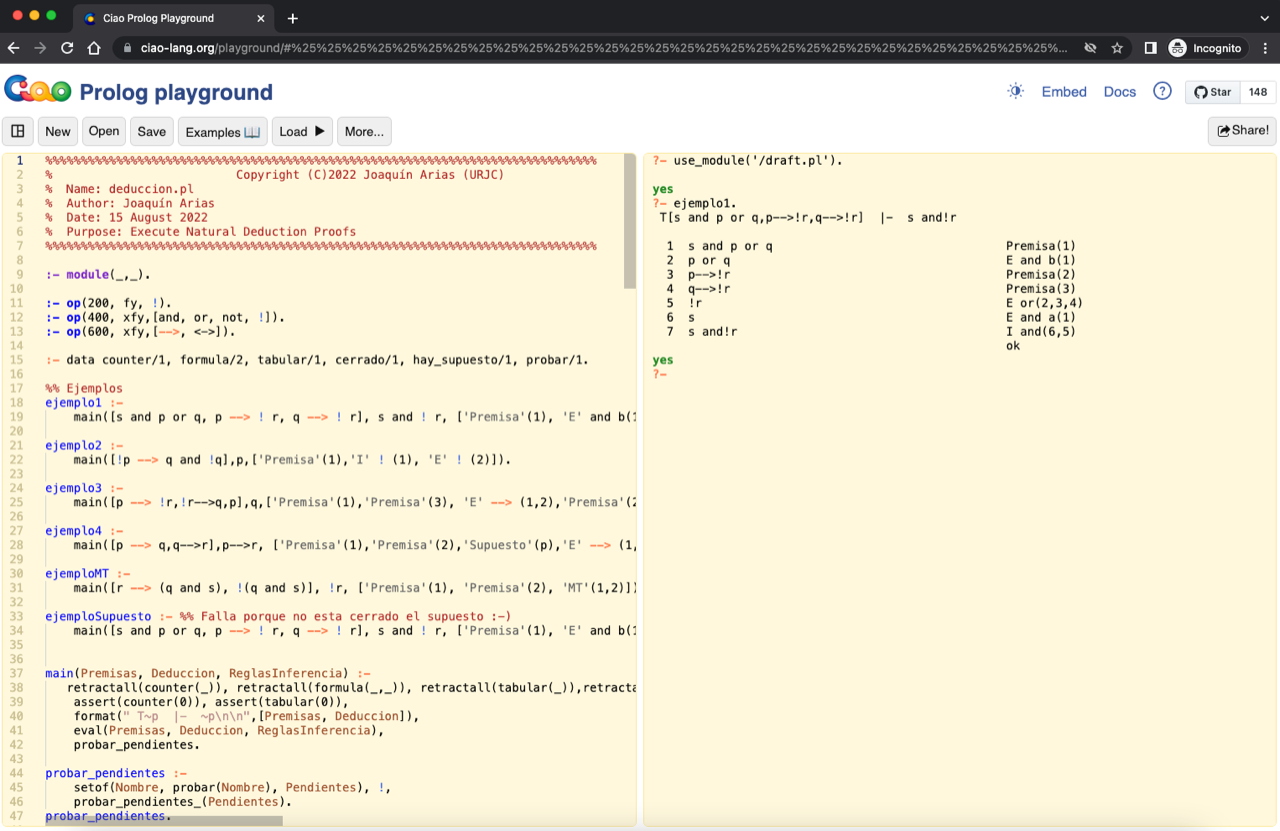
\includegraphics[scale=.3]{captura}  
  \caption{Captura de pantalla con la ejecución de \code{DeduccionNatural.pl}}
  \label{fig:ded}
\end{figure}



\section{Definir reglas derivadas}
\label{sec:derivadas}


\appendix
\printbibliography

\end{document}

